\documentclass[11pt, a4paper]{COMP3021}
\usepackage{fancyhdr}
\usepackage{setspace}
\usepackage{amsmath,mathrsfs}
\usepackage{multicol}
\usepackage{amssymb}
\usepackage{graphicx}
\usepackage{caption}
\usepackage{subcaption}
\usepackage{xcolor}
\usepackage{float}
\usepackage{tikz}
\usepackage{multirow}
\usepackage{minted}
\usepackage[linesnumbered, ruled, boxed]{algorithm2e}
\SetKwRepeat{Do}{do}{while}
\setminted[java]{breaklines,autogobble,breakanywhere,linenos,mathescape}
\setmintedinline[java]{breaklines,breakanywhere}
\newcommand{\motiv}{\blue {\bf Motivation: }}
\newcommand{\eg}{\textbf{Example. }}
\newcommand{\sol}{\red {\bf Solution. }}

\title{Topic 9}
\subtitle{Event-Driven Programming}

\begin{document}
\begin{spacing}{1.2}

    \section{Define an Event Handler}

    {\motiv Up to now, our programs are always executed in a {\it procedural}
    order, but sometimes, we need certain codes to execute {\it upon
    activation of events}, such as button presses.}

    To handle GUI events, there are two components: 
    \begin{itemize}
        \item {\bf Event Source:} like button, keyboard, etc.
        \item {\bf Event listener:} which {\it handles the event}, 
        usually a method(known as {\bf event handler})
        \begin{minted}{java}
            public void handle(ActionEvent e) {
                // what to perform when event occurs
            }
        \end{minted}
    \end{itemize}

    There are two steps to do: 
    \begin{enumerate}
        \item write a handler.
        \item create a instance of the class {\bf implements this handler},
        and {\bf register} this instance to listen to the {\bf event source}.
        \item then java will automatically call the handler when the event occurs.
    \end{enumerate}
    \eg The button is defined as follow: 
    \begin{minted}{java}
        var btOK = new Button("OK");
        var okHandler = new OKHandlerClass();
        btOK.setOnAction(okHandler);
    \end{minted}
    And the handler class is: 
    \begin{minted}{java}
        class OKHandlerClass implements EventHandler<ActionEvent> {
            @Override
            public void handle(ActionEvent e) {
                System.out.println("OK button clicked");
            }
        }
    \end{minted}
    When the button ``OK'' is pressed, the program prints ``OK button clicked''
    on the console.

    \vspace{0.5in}
    There are lots of commonly used {\bf Actions, Events} and {\bf Handlers.}
    \begin{center}
        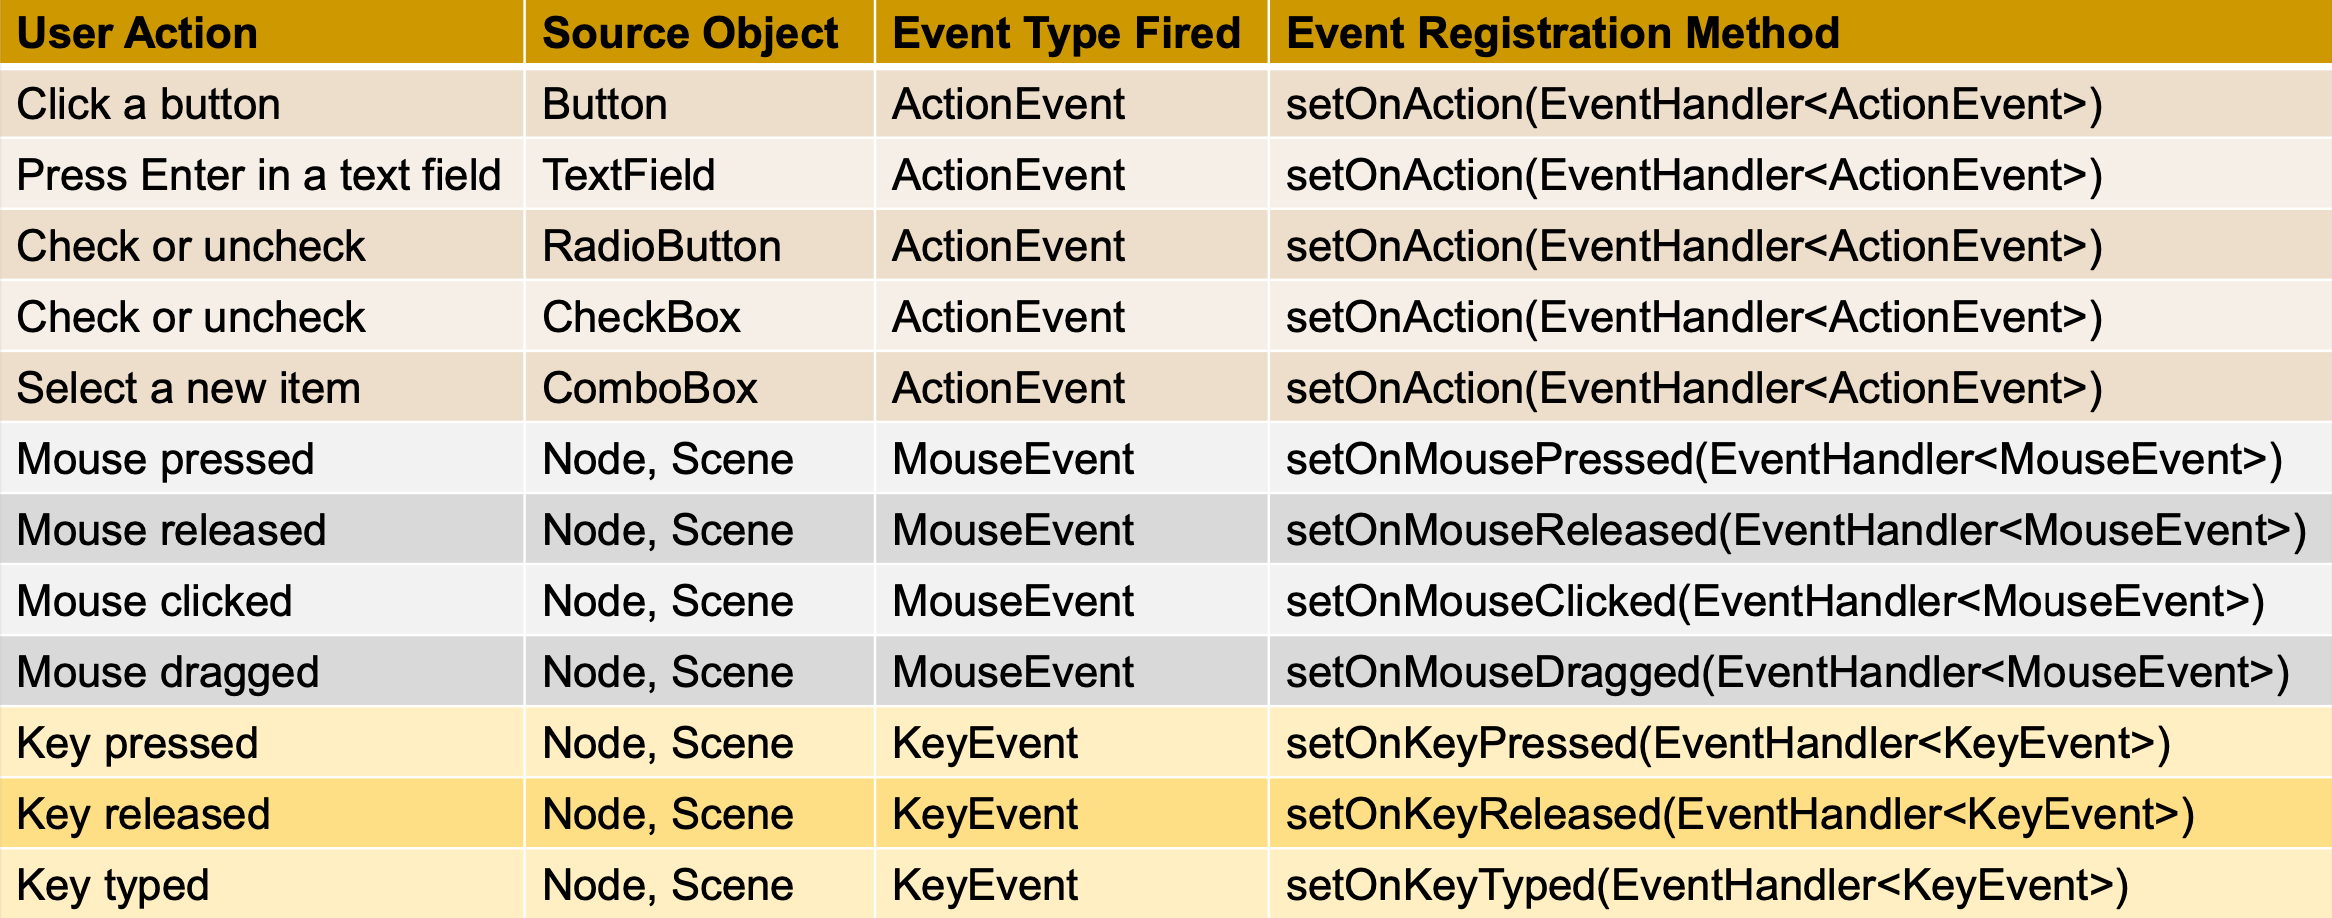
\includegraphics[scale=0.39]{images/08-events.png}
    \end{center}
    For example, if we want to listen to and handle a {\bf mouse pressed} event,
    we need to define a class that 
    \mintinline{java}{implements EventHandler<MouseEvent>}, and {\bf override}
    the \mintinline{java}{handle()} method inside.

    \vspace{0.5in}
    Below are some commonly-used Events and there hierarchy.
    \begin{center}
        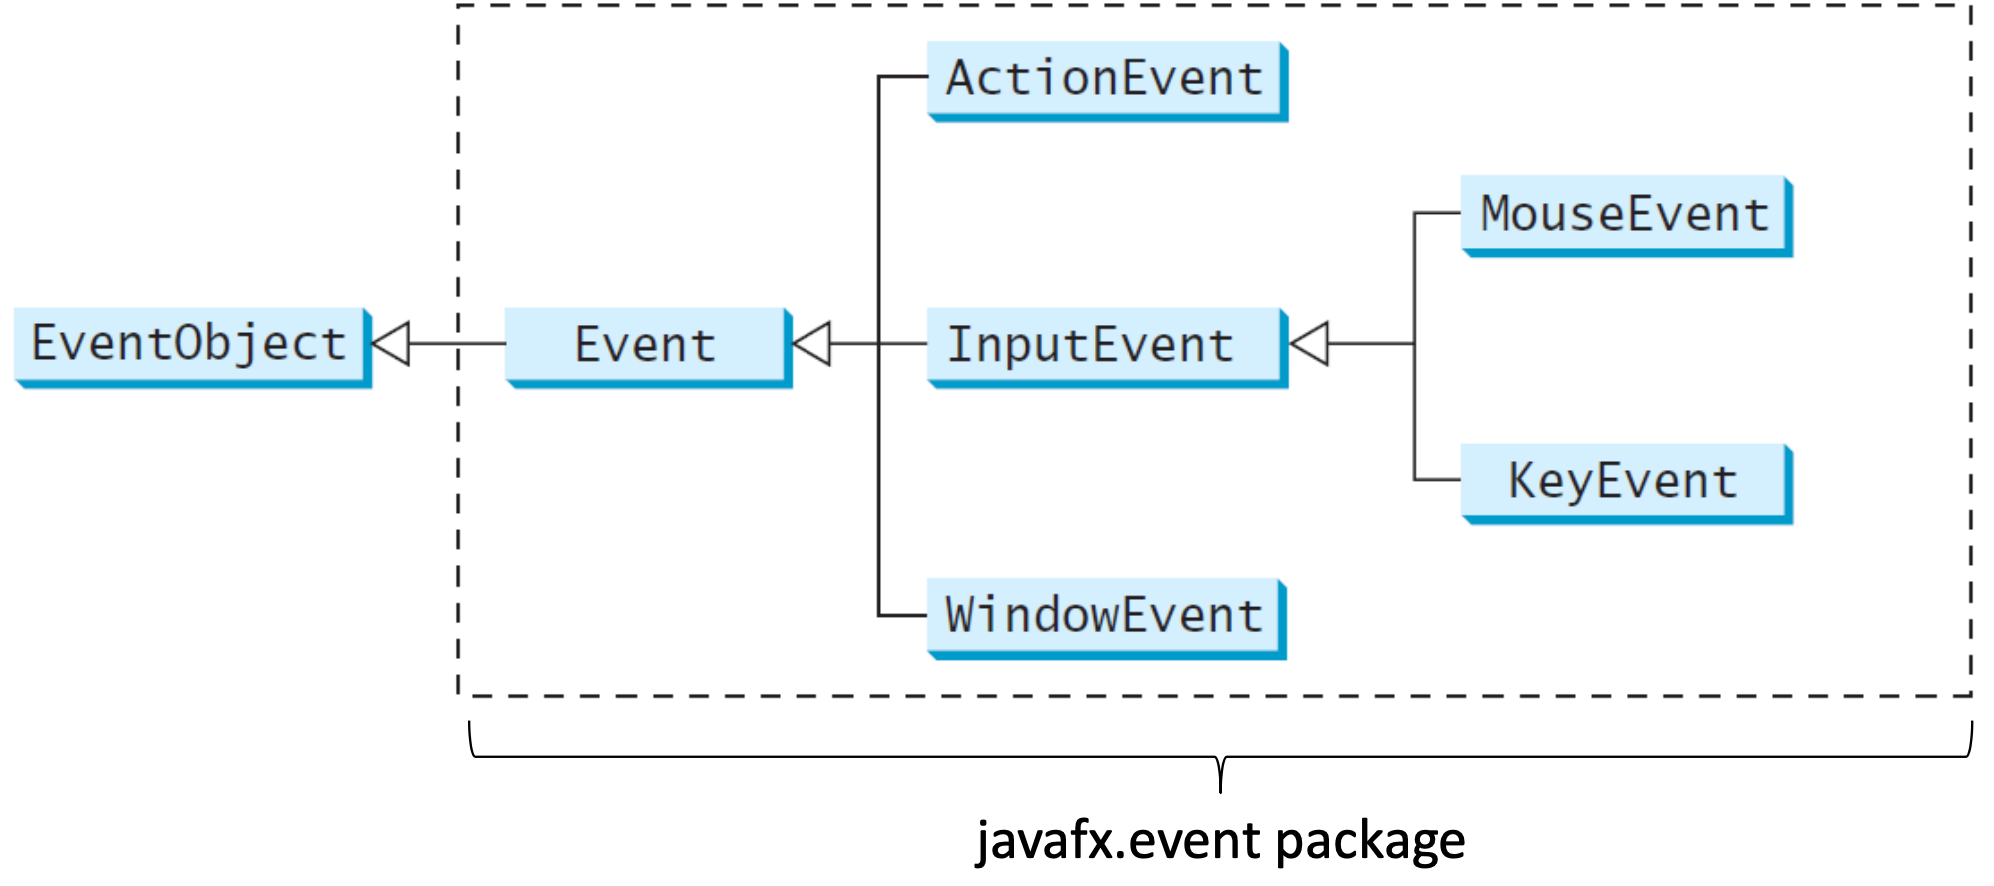
\includegraphics[scale=0.4]{images/08-events-tree.png}
    \end{center}

    The \mintinline{java}{EventHandler<T extends Event>} interface accepts 
    type {\bf T} that is a subtype of {\bf Event} class.


    \newpage
    \section{Inner Class}
    {\motiv 
        Mostly, an event handler is {\it exclusively owned by an application},
        which means it's {\it improper to be accessible by other applications}.
        Thus {\bf inner class} is introduced.
    }

    An {\bf inner class} is a {\bf non-static} class defined inside another class.
    {\bf Note: }we can only declare \mintinline{java}{protected, private} class in 
    inner class. When we define an inner class as ``private'', it means {\it only 
    its outer class can access it}, even the class in same package {\it cannot}.
    \begin{minted}{java}
        public class MyFXApplication extends Application {
            private int data = 3021;
            @Override
            public void start(Stage primaryStage) {
                var btOK = new Button("OK");
                btOK.setOnAction(new MyListener());
                // ...
                System.out.println("i = " + new MyListener().i);    // can access var in inner class
            }
            // Inner class, exclusively owned by MyFXApplication
            private class MyListener implements EventHandler<ActionEvent> {
                private int i = 0;
                @Override
                public void handle(ActionEvent event) {
                    i = data;     // can access to var in outer class
                    System.out.println(i);
                }
            }
        }
    \end{minted}

    Notice when {\bf outer class} access to instance variables in {\bf inner class}, we need 
    to create an instance of inner class first, but when {\bf inner class} access 
    to instance variables in {\bf outer class}, there is no need to do so, 
    since one outer class instance {\it must have been created before} the inner class 
    exists, and in this situation, {\it Inner class uses the \textbf{current snapshot} 
    of the Outer class.}


    \newpage
    \section{Accessability of Inner Class}

    {\bf Inner Class} and {\bf Outer Class} are ``friends'' {\it in both directions},
    which means they can access to the other's private members.

    [{\it Compare with C++}: The ``friend'' mechanism in C++ breaks the rule of 
    encapsulation, and lots of ``friend'' relationships make it messy for other 
    team members to maintain the code.]
    
\end{spacing}
\end{document}
